%% LaTeX-Beamer template for KIT design
%% by Erik Burger, Christian Hammer
%% title picture by Klaus Krogmann
%%
%% version 2.1
%%
%% mostly compatible to KIT corporate design v2.0
%% http://intranet.kit.edu/gestaltungsrichtlinien.php
%%
%% Problems, bugs and comments to
%% burger@kit.edu

\documentclass[18pt]{beamer}

%% SLIDE FORMAT

% use 'beamerthemekit' for standard 4:3 ratio
% for widescreen slides (16:9), use 'beamerthemekitwide'

\usepackage{templates/beamerthemekit}
\usepackage[utf8]{inputenc}
% \usepackage{templates/beamerthemekitwide}

%% TikZ INTEGRATION

% use these packages for PCM symbols and UML classes
\usepackage{templates/tikzkit}
% \usepackage{templates/tikzuml}
\usepackage{listings}
\usepackage{tabulary}
\usepackage{pgfplots}
\usepackage{tikz}
\usetikzlibrary{positioning,matrix,graphs,arrows,patterns,shapes,external,calc,fit,backgrounds}

\selectlanguage{ngerman}

\title[Treppenerkennung für einen treppensteigenden Roboter]{Treppenerkennung für einen treppensteigenden Roboter}
\subtitle{Projektpraktikum Robotik und Automation I (Software)}
\author{Maximilian Heß}

\institute{Institut für Anthropomatik und Robotik (IAR) - Intelligente Prozessautomation und Robotik (IPR)}

% Bibliography

\usepackage[citestyle=authoryear,bibstyle=numeric,hyperref,backend=biber]{biblatex}
\addbibresource{templates/example.bib}
\bibhang1em

\begin{document}

%title page
\begin{frame}
	\titlepage
\end{frame}

%table of contents
\begin{frame}{Übersicht}
	\tableofcontents
\end{frame}



\section{Motivation}

\begin{frame}{Motivation}
\begin{itemize}
	\item Langfristiges Ziel: Exploration über mehrere Stockwerke
	\begin{itemize}
		\item Ermöglicht die Einführung von Ebenen in 2D-Karten
		\item Verknüpfung der Ebenen mittels Treppenmarkierungen
		\item Anwendungsbeispiel: Wegfindung über mehrere Stockwerke
	\end{itemize}
	\item Kurzfristiges Ziel: Finden und Kartografieren von Treppen (Ziel des Praktikums)
\end{itemize}
\end{frame}



\section{Hintergrund}

\subsection{Roboterplattform - HMMWV}
\begin{frame}{Roboterplattform - HMMWV}
\begin{itemize}
	\item Sick LMS 100 (LiDAR)
	\item BRIX mit Intel i5 vierter Generation (Intel Core i5-4570R @ 2.70GHz)
	\item Asus Action Camera für 3D-Erfassung der Umgebung
\end{itemize}
\begin{center}
	\includegraphics[scale=0.3]{images/hmmwv.jpg}
\end{center}
\end{frame}


\subsection{Robot Operating System (ROS)}
\begin{frame}{Robot Operating System (ROS)}
\begin{columns}
	\column{0.5\textwidth}
	\begin{itemize}
		\item Verteilte Middleware zur Automatisierung der Kommunikation der Robotern-Komponenten
		\item Zentrale Aufgaben
		\begin{itemize}
			\item Nachrichtenaustausch (zentraler Broker, Publisher-Subscriber-Prinzip)
			\item Hardwareabstraktion
		\end{itemize}
		\item Viele Komponenten für Standardaufgaben (z.B. für SLAM, Sensoren, etc.)
	\end{itemize}
	\column{0.3\textwidth}
		\vspace{10px}
		\includegraphics[scale=0.04]{images/rosgraph_hmmwv.pdf}
\end{columns}
\end{frame}



\section{Theoretische Vorüberlegungen}

\subsection{Ansatz 1: Erkennen von Treppen mittels horizontaler Linien }
\begin{frame}{Ansatz 1: Erkennen von Treppen mittels horizontaler Linien}
\begin{itemize}
	\item Canny-Algorithmus zur Kantenerkennung
	\item Eingabe: Tiefenbild von Asus Xtion Kamera
\end{itemize}
\begin{columns}
	\column{0.25\textwidth}
	\includegraphics[scale=0.16]{images/canny00.pdf}\newline
	\includegraphics[scale=0.16]{images/canny02.pdf}
	\column{0.25\textwidth}
	\includegraphics[scale=0.16]{images/canny01.pdf}\newline
	\includegraphics[scale=0.16]{images/canny03.pdf}
\end{columns}
\end{frame}


\subsection{Ansatz 2: Erkennen von Treppen mittels vertikaler Flächen}
\begin{frame}{Ansatz 2: Erkennen von Treppen mittels vertikaler Flächen}
\begin{itemize}
	\item Eingabe: drei-dimensionale Punktwolke
	\item Verwendung des RANSAC-Algorithmus zur Ermittlung von Flächen (dazu gleich mehr)
\end{itemize}
\begin{center}
	\includegraphics[scale=0.13]{images/screenshot_pointcloud.png}
\end{center}
\end{frame}

\begin{frame}{RANSAC-Algorithmus}
\begin{itemize}
	\item Problem: Automatisch erfasste Messdaten enthalten meist viele Ausreißer
	\item RANSAC: Modellbasiertes Schätzen, welche Punkte zur Zielmenge gehören
	\item Eingabe
	\begin{itemize}
		\item Modell einer senkrechten Fläche (Stufenvorderseiten)
		\item Punktwolke
	\end{itemize}
\end{itemize}
\end{frame}


\section{Implementierung}

\begin{frame}{Implementierung}
\begin{itemize}
	\item ROS Node zur Treppenerkennung
	\item C++, PCL
	\item Einführen Formats zur Speicherung der Treppen
	\begin{itemize}
		\item YAML
	\end{itemize}
	\item Import-/Export-Funktionen mittels \texttt{rosservice}
\end{itemize}
\end{frame}

\begin{frame}{Implementierung im Detail}
\begin{itemize}
	\item Eingabe: Punktwolke, Ausgabe: Liste mit Treppen
\end{itemize}
\begin{center}
	\includegraphics[scale=0.42]{activitydiagram.pdf}
\end{center}
\end{frame}

\begin{frame}{Implementierung im Detail}
\begin{itemize}
	\item Nach Anwendung von \texttt{RANSAC}: Erkennen von senkrechten Flächen
\end{itemize}
\begin{center}
	\includegraphics[scale=0.16]{images/ransac01.pdf}
\end{center}
\end{frame}

\begin{frame}{Implementierung im Detail}
\begin{itemize}
	\item Höhenfilter
\end{itemize}
\begin{center}
	\includegraphics[scale=0.16]{images/ransac02.pdf}
\end{center}
\end{frame}

\begin{frame}{Implementierung im Detail}
\begin{itemize}
	\item Treppenbauen
\end{itemize}
\begin{center}
	\includegraphics[scale=0.16]{images/ransac03.pdf}
\end{center}
\end{frame}

\begin{frame}{Video}
\begin{center}Video\end{center}
\end{frame}

\begin{frame}[fragile]
\frametitle{Speicherformat für Import/Export}
\begin{itemize}
	\item \texttt{rosservice call export\_stairways stairs.yaml}
	\item Beipiel
\end{itemize}
\begin{center}
	\begin{lstlisting}
	stairways:
	  - step_height: 0.1944063454866409
	    step_depth: 0.2506448223569446
	    step_width: 0.8087717592716217
	    stairway_height: 0.5734314657747746
	    step_count: 3
	    first_step:
	      y: 0.04630382890261724
	      z: 0.200202414393425
	      x: 1.063629030461962

	\end{lstlisting}
\end{center}
\end{frame}



\section{Bewertung des Ergebnisses}

\begin{frame}{Bewertung des Ergebnisses}
\begin{itemize}
	\item Beispieltreppe im Poolraum wird zuverlässig erkannt \(\longrightarrow\) Ziel erreicht
	\item Probleme/Schwächen
	\begin{itemize}
		\item Nur für sehr kurze Distanzen geeignet
		\begin{itemize}
			\item Kein Treppenmodell als Eingabe
			\item Reichweite der Kamera
		\end{itemize}
		\item Hohe Hardware-Anforderungen zur Verarbeitung der Punktwolken
	\end{itemize}
\end{itemize}
\end{frame}

\begin{frame}{Laufzeit des Algorithmus}
\begin{columns}
	\column{0.5\textwidth}
	\begin{itemize}
		\item CPU: Intel Core i5-4570R @ 2.70GHz, 4 Kerne, kein HT
		\item Algorithmus nicht parallelisiert
	\end{itemize}
	\column{0.5\textwidth}
	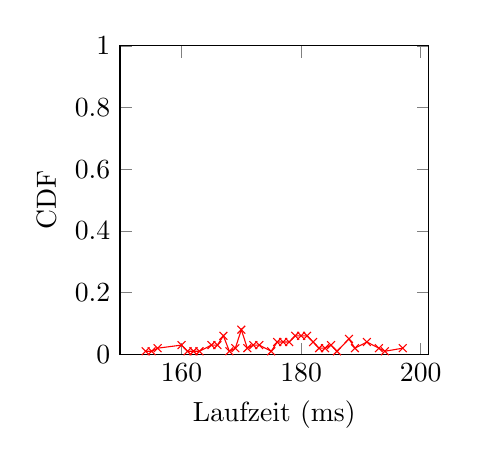
\begin{tikzpicture}
        \begin{axis}[
            width=5.5cm,
            height=5.5cm,
            xlabel=Laufzeit (ms),
            ylabel=CDF, ymin=0, ymax=1.0,
            tick label style={/pgf/number format/fixed}]
           \addplot[color=red,mark=x] coordinates {
           		(154, 0.01) (155, 0.01) (156, 0.02)
                (160, 0.03) (161, 0.01) (162, 0.01) (163, 0.01) (165, 0.03) (166, 0.03) (167, 0.06) (168, 0.01) (169, 0.02)
                (170, 0.08) (171, 0.02) (172, 0.03) (173, 0.03) (175, 0.01) (176, 0.04) (177, 0.04) (178, 0.04) (179, 0.06)
                (180, 0.06) (181, 0.06) (182, 0.04) (183, 0.02) (184, 0.02) (185, 0.03) (186, 0.01) (188, 0.05) (189, 0.02)
                (191, 0.04) (193, 0.02) (194, 0.01) (197, 0.02)
           };
    	\end{axis}
    \end{tikzpicture}
\end{columns}
\end{frame}

\begin{frame}{Ausblick}
\begin{itemize}
	\item Langzeitvision: Verknüpfen mehrerer Kartenabschnitte durch Treppen
	\begin{itemize}
		\item Beispielsweise Stockwerke (eine Karte pro Stockwerk)
	\end{itemize}
	\item Einfügen eines geeigneten Treppenmodells
\end{itemize}
\end{frame}

\end{document}
